% Important: If latex complains about unicode characters,
% please use "\usepackage[utf8x]{inputenc}" in your preamble
% You can change the size of the picture by putting it into the construct:
% 1) \resizebox{10cm}{!}{"below picture"} to scale horizontally to 10 cm
% 2) \resizebox{!}{15cm}{"below picture"} to scale vertically to 15 cm
% 3) \resizebox{10cm}{15cm}{"below picture"} a combination of above two
% It is not recomended to use the scale option of the tikzpicture environment.
\scalebox{1}{
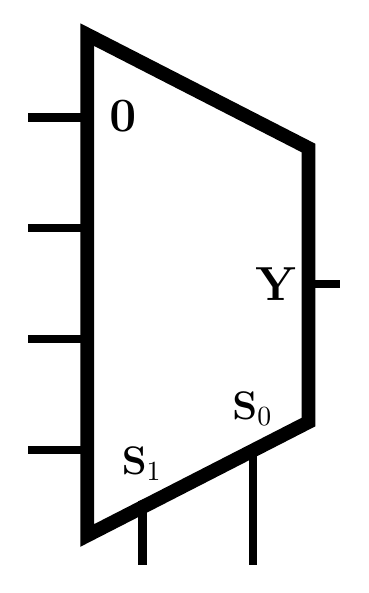
\begin{tikzpicture}[x=1pt,y=-1pt,line cap=rect]
\def\logisimfontA#1{\fontfamily{cmr}{#1}} % Replaced by logisim, original font was "SansSerif"
\def\logisimfontB#1{\fontfamily{CMU Sans Serif}{#1}}
\definecolor{custcol_0_0_0}{RGB}{0, 0, 0}
\definecolor{custcol_ff_ff_ff}{RGB}{255, 255, 255}
\draw [line width=3.0pt, custcol_0_0_0 ]  (45.0,175.0) -- (45.0,195.0) ;
\draw [line width=3.0pt, custcol_0_0_0 ]  (105.0,95.0) -- (115.0,95.0) ;
\draw [line width=3.0pt, custcol_0_0_0 ]  (85.0,155.0) -- (85.0,195.0) ;
\draw [line width=3.0pt, custcol_0_0_0 ]  (5.0,35.0) -- (25.0,35.0) ;
\draw [line width=3.0pt, custcol_0_0_0 ]  (5.0,75.0) -- (25.0,75.0) ;
\draw [line width=3.0pt, custcol_0_0_0 ]  (5.0,115.0) -- (25.0,115.0) ;
\draw [line width=3.0pt, custcol_0_0_0 ]  (5.0,155.0) -- (25.0,155.0) ;
\fontsize{16pt}{16pt}\fontseries{bx}\selectfont\node[inner sep=0, outer sep=0, custcol_0_0_0, anchor=base west] at  (85.75,101.0)  {\textbf{Y}};
\draw [line width=5.0pt, custcol_0_0_0 ]  (25.0,5.0) -- (25.0,186.0) -- (105.0,145.0) -- (105.0,46.0) -- cycle;
\fontsize{14pt}{14pt}\fontseries{bx}\selectfont\node[inner sep=0, outer sep=0, custcol_0_0_0, anchor=base west] at  (77.5,144.0)  {\textbf{S$_0$}};
\fontsize{16pt}{16pt}\fontseries{bx}\selectfont\node[inner sep=0, outer sep=0, custcol_0_0_0, anchor=base west] at  (33.0,40.0)  {\textbf{0}};
\fontsize{14pt}{14pt}\fontseries{bx}\selectfont\node[inner sep=0, outer sep=0, custcol_0_0_0, anchor=base west] at  (37.5,164.0)  {\textbf{S$_1$}};
\fill [line width=1.0pt, custcol_0_0_0]  (25.0,35.0) ellipse (2.0 and 2.0 );
\fill [line width=1.0pt, custcol_0_0_0]  (25.0,75.0) ellipse (2.0 and 2.0 );
\fill [line width=1.0pt, custcol_0_0_0]  (25.0,115.0) ellipse (2.0 and 2.0 );
\fill [line width=1.0pt, custcol_0_0_0]  (25.0,155.0) ellipse (2.0 and 2.0 );
\fill [line width=1.0pt, custcol_0_0_0]  (45.0,175.0) ellipse (2.0 and 2.0 );
\fill [line width=1.0pt, custcol_0_0_0]  (85.0,155.0) ellipse (2.0 and 2.0 );
\fill [line width=1.0pt, custcol_0_0_0]  (105.0,95.0) ellipse (2.0 and 2.0 );
\end{tikzpicture}
}
